%!BIB program = bibtex
\documentclass[9pt, twocolumn, twoside, lineno]{pnas-new}
% Use the lineno option to display guide line numbers if required.

% PNAS研究论文模板
\templatetype{pnasresearcharticle} % Choose template 
% {pnasresearcharticle} = Template for a two-column research article
% {pnasmathematics} %= Template for a one-column mathematics article
% {pnasinvited} %= Template for a PNAS invited submission
% \usepackage{cite}
\usepackage{url}	
% 文章标题:“流域尺度的水资源利用体系:过渡框架和发展困局”
\title{Regime transition identification for basin's governance challenges of water use}
\label{title}
% Use letters for affiliations, numbers to show equal authorship (if applicable) and to indicate the corresponding author
% 作者列表
\author[a, b]{Shuang Song}  % 宋爽,一作
\author[a, b, 1]{Shuai Wang}  % 王老师,通讯
\author[c, d]{Xutong Wu}  % 武旭同
\author[e]{Yongping Wei} % 尉老师
\author[a, b]{Bojie Fu}  % 傅老师

% 机构列表
\affil[a]{ % 北师大地表国重
	State Key Laboratory of Earth Surface Processes and Resource Ecology, 
	Faculty of Geographical Science, 
	Beijing Normal University, 
	Beijing 100875, 
	P.R. China
}
\affil[b]{ % 北师大地理学部
	Institute of Land Surface System and Sustainability, 
	Faculty of Geographical Science, 
	Beijing Normal University, 
	Beijing 100875, 
	P.R. China
}
\affil[c]{ % 北大城环
	College of Urban and Environmental Sciences, 
	Peking University, 
	Beijing 100871, 
	P.R. China
}
\affil[d]{ % 中科院生态中心
	State Key Laboratory of Urban and Regional Ecology, 
	Research Center for Eco-Environmental Sciences, 
	Chinese Academy of Sciences, 
	Beijing 100085, 
	P.R. China 
}
\affil[e]{ % 昆士兰大学
	School of Earth and Environmental Sciences, 
	The University of Queensland, 
	Brisbane 4067, 
	Australia
}

% Please give the surname of the lead author for the running footer
% 领衔作者
\leadauthor{Song} 

% Please add a significance statement to explain the relevance of your work
% PNAS特有的“Significance陈述”,用不超过120个字来说明研究的意义和亮点
\significancestatement{
\label{significance}
	% Authors must submit a 120-word maximum statement about the significance of their research paper written at a level understandable to an undergraduate educated scientist outside their field of speciality. The primary goal of the significance statement is to explain the relevance of the work in broad context to a broad readership. The significance statement appears in the paper itself and is required for all research papers.
	It is a well-known fact that development of human societies backs on water use.
	Therefore, as natural water cycle has been dominated by growing socio-economic processes, big river basins are roundly governed stage by stage for further water use. 
	We propose a new method with an integrated index to detect water governance regimes and applying it to the Yellow River Basin, a typical fast-changing basin in China.
	Since our index integrates various considerations of water governance (who gets what water, when and how), a widespread regime transition schema can be summarized after then. 
	By identifying governance challenges, the schema can be a useful guideline for basins all around the world in their sustainable developing trajectories. 
}

% Please include corresponding author, author contribution and author declaration information
\authorcontributions{ % 作者的相应贡献
	Shuai Wang and Bojie Fu designed this research,
	Shuang Song performed the research and analysed data,
	Shuang Song, Xutong Wu wrote the paper.
	Yongping Wei reviewed the manuscript and proposed major useful advices.
}
\authordeclaration{ % 利益冲突陈述
	The authors declare no competing interests.
}

% 如果有共同一作的情况,则uncomment下面这行代码的注释
%\equalauthors{\textsuperscript{1}A.O.(Author One) contributed equally to this work with A.T. (Author Two) (remove if not applicable).}

% 通讯作者信息
\correspondingauthor{\textsuperscript{1}To whom correspondence should be addressed. E-mail: shuaiwang@bnu.edu.cn}

% 关键词,三到五个
% At least three keywords are required at submission. Please provide three to five keywords, separated by the pipe symbol.
\keywords{Regime shifts $|$ Water use $|$ Water governance $|$ Socio-hydrology $|$ Sustainability} 

%tag 摘要
% 为了
\begin{abstract}
	\label{abstract}
	% 为了持续的社会经济发展,人类治理了大型河流,并在世界范围内引发了一系列流域尺度的稳态转换。
	For water uses in sustaining socio-economic development, human have governed large rivers and triggered various regime shifts at a basin scale all around the world. 
	% 由于水治理制度决定谁、何时和如何获得水,因此确定其过渡对于指导有效和可持续的用水至关重要。
	Since water governance regime decides who gets what water, when and how much, identification for its changes is critical to guiding efficient and sustainable water uses.
	% 在这里,考虑到水治理的三个主要维度(压力、供应和分配),我们开发了一个流域尺度上的综合水治理指数(IWGI),以检测制度的变化。
	Here, considering three main dimensions of water governance (storage, provision and allocation), we develop an Integrated Water Governance Index (IWGI) at a basin scale to detect regime shifts.
	% 将该指数应用于中国黄河流域,可以看出,在过去半个多世纪中,有三个政权的转变是由经济增长、管理和效率提高引起的。  
	By applying this index to the Yellow River Basin, China, it suggests there were two regimes shifts of water governance throughout half a century, which were caused by environmental, economic social and political changes.
	% 在此基础上,我们总结了一个与水社会循环相对应的一般制度变迁模式。
	Based on these, we summarized a widespread regime transition schema, corresponding with trajectories of water uses towards hydro-social cycle.
	% 由于资源挑战和结构挑战主要困扰不同制度下的水治理,这一过渡模式可以作为协调大流域治理的有益指导。
	Since different governance challenges mainly occurred at different stages in transition, this schema can be a useful guideline for governing big river basins in a coordinated way.
\end{abstract}


\dates{This manuscript was compiled on \today}
\doi{\url{www.pnas.org/cgi/doi/10.1073/pnas.XXXXXXXXXX}}


\begin{document}

\maketitle
\thispagestyle{firststyle}
\ifthenelse{\boolean{shortarticle}}{\ifthenelse{\boolean{singlecolumn}}{\abscontentformatted}{\abscontent}}{}
% If your first paragraph (i.e. with the \dropcap) contains a list environment (quote, quotation, theorem, definition, enumerate, itemize...), the line after the list may have some extra indentation. If this is the case, add \parshape=0 to the end of the list environment.

\label{introduction-section-1}
% 水资源在人类世的重要性,是支持人类社会发展的基础。
\dropcap{W}ater, at “the centre of the planetary drama of the Anthropocene”, is not only essential for Earth system processes, but also supporting development of human societies. 
%* add references
% 然而,根据人类用水的需求,人类的改造对自然水循环产生了深远的影响,并将其发展轨迹逐步推向了水社会循环。
Because of relying on water use, human activities have profoundly modified the natural water cycle and led the trajectory towards a hydro-social water cycle, stage by stage
\cite{gleesonIlluminatingWaterCycle2020,cummingLinkingEconomicGrowth2018}.
% 面对人类世世的重大转变,世界许多大河流域,也是经济和文明的热点地区,迫切需要成功的治理以实现可持续发展
Facing this major transformation in the Anthropocene, many of the world's big river basins, also hot spots of economy and civilization, are urgently in need of successful governance for sustainable water use
\cite{bestAnthropogenicStressesWorld2019}. 
% 作为地球系统治理框架的一个组成部分,水治理需要对人类社会和水资源利用之间的复杂关系有深刻的理解。
As an integral part of a proposed Earth system governance framework, water governance requires deep understanding of the complex relationships between human societies and water use.
% Biermann et al., 2012.
% 因此在流域尺度上,识别由向水-社会水循环的转变所引起的变化是至关重要的。
Therefore, it is crucial to identify changes of water governance induced by the transformation towards hydro-social water cycle, at a basin scales.

\label{introduction-section-2}
% 缺乏治理就是缺乏可持续性
On the trajectory of development, missing governance means missing sustainability.
% 根据联合国开发计划署(UNDP)的说法,水管理决定了用水的三个关键方面:“有多少水可供使用?、“如何平衡用水服务?”“以及‘如何平等有效地分配水资源?’”
According to United Nations Development Programme (UNDP), three key dimensions of water use are decided by a water governance regime directly: ``How much water can be used? (storage)'', ``How to balances different water use services? (provision)'' and ``How to allocate water equally and efficiently? (allocation)''.
% Regime 和 Regime shift 的定义。
Regime is a stable state of system’s structure and function, of which large and persistent changes may lead to substantive impacts on the outcomes of system with widespread cascading effects, defined as regime shifts 
\cite{rochaCascadingRegimeShifts2018,schefferCatastrophicRegimeShifts2003, schefferCatastrophicShiftsEcosystems2001}.
% 因此,确定关于水治理的制度变化是重要的,它标志着水资源利用的实质性变化,并导致可持续性方面的新的治理挑战。
Identification of regime shifts regarding water governance, therefore, is important as a signal of substantive change in water use and lead to new governance challenges in sustainability.
% 随着环境、经济、社会和政策情况。
Changed with environmental, economic, social and political situation, the three dimensions may compose various water governance regimes. 
% 首先,受环境恶化和经济发展用水的影响,水资源短缺会增加社会的压力,但水库建设等管理政策有助于缓解压力。
Firstly, effected by environment deteriorate and demands of further economic development, maintaining storage for societies can face stress because of water scarcity, but governance policies (such as construction of reservoirs for storage) are helpful to relief
\cite{postelHumanAppropriationRenewable1996, greveGlobalAssessmentWater2018, qinFlexibilityIntensityGlobal2019}.
% 其次,在供应用水(如家庭用水和粮食生产用水)和非供应用水(如工业生产或能源用水)之间存在权衡,这需要由治理制度来平衡。
Secondly, there is trade-off between provisioning water use (such as domestic use and food production uses) and non-provisioning water (such as uses for industrial production or energy), which in need of considerations through water governance
\cite{liuWaterScarcityAssessments2017, florkeWaterCompetitionCities2018}.
% 第三,由于配置是流域关注的问题,它不仅受到区域环境基础的影响,而且还受到区域经济比较优势的影响,而经济比较优势可能受到社会发展和政策的影响。
Thirdly, since allocation is a concern of the whole basin, it not only influenced by regional environmental foundations, but also changed by regions' economic comparative advantages, which is easily changed by social development and policies.
% 总的来说,用水治理决定了与用水的“压力”、“供给”和“分配”,而三者在用水转向社会-水循环的过程中都发生着不断的变化
Taken together, along with the transformation towards a human-dominated hydro-social water cycle, water governance regimes determined by three changing dimensions (storage, provision and allocation), and it is crucial to identify their shifts in a simple but comprehensive way for basins' sustainability (Figure~\ref{fig:framework}).

\label{introduction-section-3}
% 黄河流域(YRB,见\textit{ Appendix}方法S1),在中国经历了最激烈的水资源开发和最剧烈的管理制度变化。
The Yellow River Basin (YRB, see \textit{Appendix} Methods S1 for details) had experienced the most intense water use and dramatic shifts of regime in China, with extraordinary challenges to water governance since ancient times.
% 对1960年以前的中国,黄河巨大的含沙量不仅给YRB带来了洪泛灾害,更为利水带来巨大困难。
Half century ago, the huge sediment loads of the Yellow River in China not only brought disasters, but also made it difficult for water use. 
% 随着水保措施、水库调水调沙、修堤等治理措施的落实才得到了有效遏制。
Since 1960s, with implementations of conservation policies, regulation reservoirs, and levees constructions, these issues were effectively contained.
% 但随之而来的是越来越严重的断流,为水治理带来了新的挑战。 
However, serious drying up of the Yellow River led new challenges to governance and promoted a range of related policies to deal with.
% 如今,黄河流域仍面临严峻的治理挑战,因为区域的用水需求仍很难被全盘满足,而必须做出权衡。
Today, as water demands are still difficult to be completely met and various trade-offs must be involved between regions and sectors, there is still a long way towards successful water governance.
% 总之,随着人类影响逐步加大,为了应对层出不穷的治理挑战,黄河流域水治理发生的迅猛转变堪称世界之最。
All in all, the transformation of the YRB has been the most rapid in the world in responses to the endless governance challenges induced by environmental, economic, social or political factors.
% 因此如果能理解黄河水治理稳态的转换过程,其模式能为世界大河流域用水的可持续提供见解。
Therefore, identifying the regime shifts with challenges regarding water governance for YRB can provide insights for the world's fast-changing big river basins in their sustainable development.

\label{introduction-section-3}
% tag 引言最后一段
% 这里我们整合了三个方向,提出了描绘流域人水关系的指数
Here, by integrating three above mentioned key dimensions of water governance, we develop an Integrated Water Governance Index (IWGI) at a basin scale to indicate changes of basin's water governance (Figure~\ref{fig:framework}).
% 使用案例研究
Then, by applying this index to the YRB, we analysed the regimes shifts of water governance and their main causes, in this typical basin of rapidly changes.
% 最后总结出一般性框架
Finally, we summarized a general regime transition schema, echoing to the different challenges in water governance, which can be a useful guideline for basins to develop in a coordinated way.


\begin{figure*}%[htbp]
	\centering
	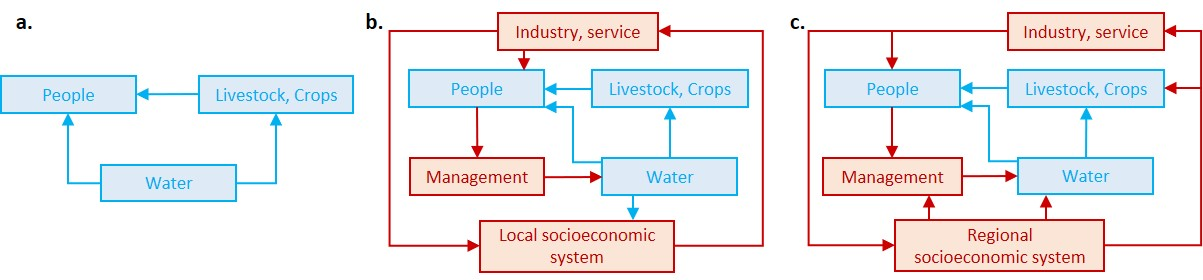
\includegraphics[width=0.8\linewidth]{../../figures/main/framework.jpg}
	\caption{
		A framework for understanding the relationship between transformation towards hydro-social cycle and water governance regimes.
		% 图A是水资源利用的三个维度。每个维度都有两个极点(红色字表示),指示水资源利用在该轴上的两个变化方向。
		\textbf{A,} three dimensions (storage, provision and allocation) of water governance (see \textit{Appendix SI} Methods S4 for details). Each dimension has two poles (denoted in red) which indicate the two potential directions of changes along that axis. (1) Storage shifts between scarcity of water resources and abundance of water resources, which means there is shortage of water supply or not. (2) provision of water can move between provisioning services or non-provisioning services, indicating how much water were used in food supporting. (3) allocation can move between balanced or lopsided, when allocation of water resources between different sectors or regions changed. We presume that water governance regimes equally weighted by these basic dimensions, whose combination can highly relate to basin development. 
		% 图B是将三个维度结合后的变化情况。因上述三个维度随着社会发展而不断变化,其组合的水资源利用状态也不同。这个过程中当突变发生时,可能标志着水资源利用发生了稳态转换,因此我们需要一个指标来监测其变化。
		\textbf{B,} the changes after combining the three dimensions. Because the above three dimensions are changing with the trajectory towards hydro-social water cycle, their combined water governance status is also different. When abrupt change occur during this process, they may indicate a regime shift in water governance, and we propose an indicator to monitor this change.
	}
	\label{fig:framework}
\end{figure*}


\section*{Results}
\subsection*{Water governance regimes}

\begin{figure}[ht!]
	\centering
	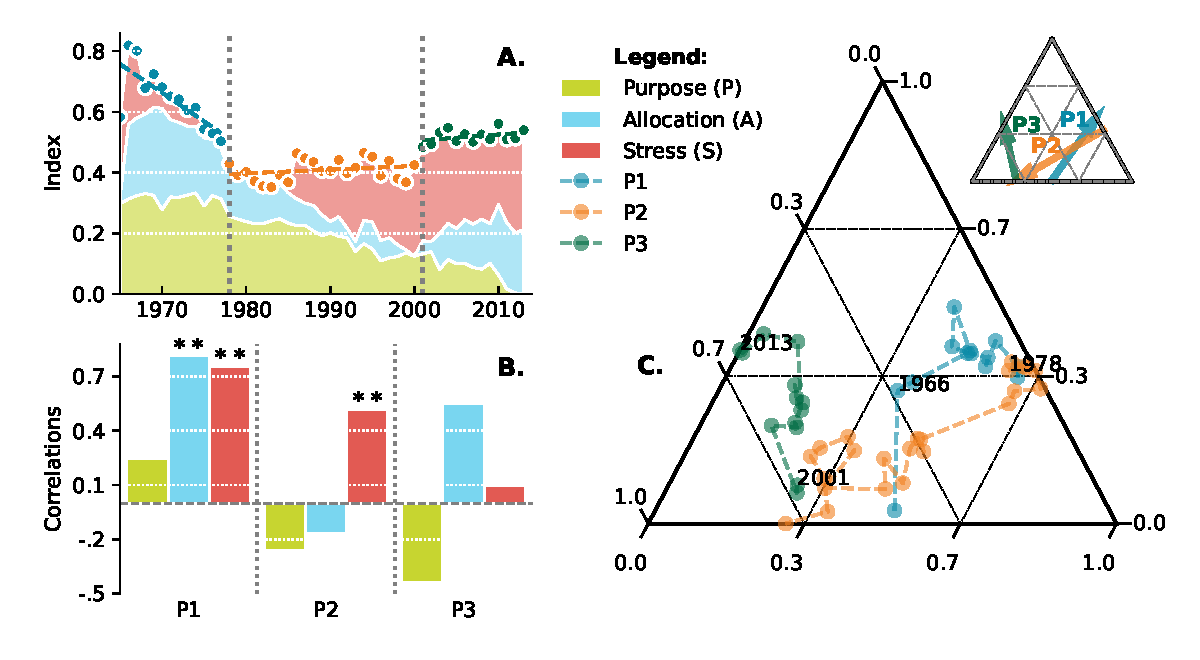
\includegraphics[width=\linewidth]{../../figures/main/index.pdf}
	\caption{Changes of the IWGI index. 
	\textbf{A,} Change points detection. With change points in 1978 and 1994, the IWGI have three periods in changing trend.
	\textbf{B,} Changing slopes of each period.
	\textbf{C,} Contributions of each dimension to the changes of IWGI within three periods. Storage, provision and allocation are the main positive contributor of P1, P2 and P3, respectively.
	}
	\label{fig:IWGI}
\end{figure}

% 这一节主要展示IWGI的变化趋势和WUR的划分
With two significant points, the changing trend of IWGI index are detected into three periods (Figure~\ref{fig:IWGI}A). 
Not only the slope of changes are various within each period, changes are also mainly contributed by different dimensions (Figure~\ref{fig:IWGI}B and Figure~\ref{fig:IWGI}C).
% 第一阶段
In the first period (P1, 1965-1978), the IWGI index had a rapidly increasing and the storage made the most striking positive contribution (131\%), while provision and allocation had slight negative contribution (-11\% and -20\%).
% 第二阶段
In the second period (P2, 1979-1994), though contributions of provision and allocation turned into positive, the IWGI index experienced a drop because declining storage plays a larger negative role (-188\% dropped than P1). 
% 第三阶段
However, as the further increasing of positive contributions of provision (75\%) and allocation (84\%), and decreases of water storage in negative contribution (-59\%) in the third period (P3, 1995-2013), a positive growth of the IWGI returned.

\begin{figure}[!htbp]
	\centering
	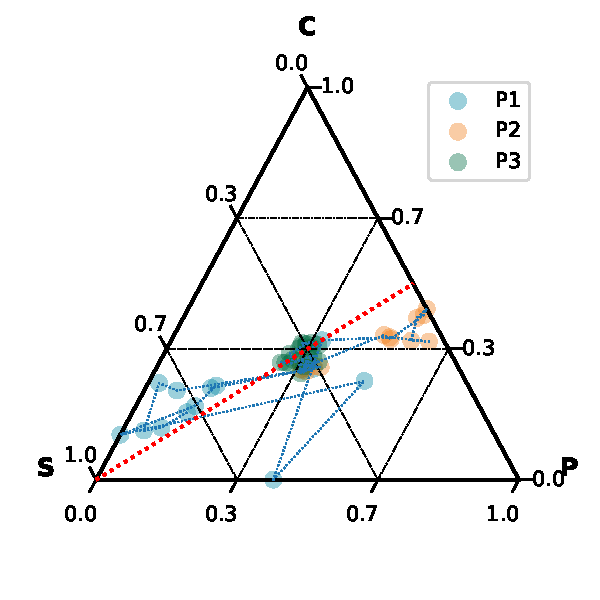
\includegraphics[width=0.9\linewidth]{../../figures/main/phases.pdf}
	\caption{Combination of contributions regards three dimensions in different periods (S: storage; P: provision; C: allocation). The closer a point to an angle of the triangle, greater the proportion of the contribution of this dimension.
	The red indicator line in this ternary plot denotes 1:1 contributions between provision (P) and allocation (C). When the points are bellow this line, the contribution ratio of allocation is lower than that of provision, and vice versa.}
	% 由于阶段一的点位于该线上方,L的净贡献比例多于P,而第二阶段的点则恰好相反。
	\label{fig:phases}
\end{figure}

% 总而言之,每个阶段都由水资源利用的不同维度提供最大的正向作用
Taken together, each period has the unique most striking positive contributor to IWGI, and overall features of three dimensions in different periods are shown in Figure~\ref{fig:phases}.
% 第一阶段到第二阶段
At the very beginning (1965) and throughout the whole P1, water governance regime dominated by increasing storage. After then, it experienced a shift to slow down in increasing storage since 1978, with a change in the proportion of contributions between provision and allocation, too.
% 第三阶段集中
Finally, the contribution of three dimensions were much similar in P3 (32.91\%, 31.87\% and 35.21\% for provision, allocation and storage respectively), making the points highly concentrated at the centre of the ternary diagram in that period.


% %tag 结果2
% \subsection*{Differences between water governance regimes}
% % 在不同的维度下各阶段进行对比,可以发现不同的水资源利用体系间存在明显差异。
% The differences between the water governance regimes are reflected in changes of all three dimensions.

% % 从阶段一到阶段二,水资源压力的变化最为明显
% Moving from the regime in P1 to P2, the most striking change is the reversal of the trend in water governance stress(Figure~\ref{fig:dimensions}A), which is determined by a combination of scarcity, flexibility and variability (Figure~\ref{fig:dimensions}D and \textit{SI Appendix} Method S4).   
% % 1. 水资源丰富,耗水量少且灵活用水
% In the P1, natural surface water resources were rather abundant with fewer water consumptions (\textit{SI Appendix} Fig. S3) and most of which were flexible water governance (\textit{SI Appendix} Fig. S4). During the P1 and even P2, however, water consumption increases rapidly and natural surface water resources decreases at the same time, making water increasingly scarce. Opposite effect to that, numerous reservoirs built reduced the variability of water resources by boosting storage capacities, but there are much fewer reservoirs built in P2 (\textit{SI Appendix} Fig. S5). As a result, water governance stress decreases during P1, but begins to rise rapidly in P2.

% % 另一方面,P2-P3,持续变化的水资源利用倾向与格局
% On the other hand, as the most positive contributors to the IWGI index in P2 and P3 separately, provision (Figure~\ref{fig:dimensions}B) and allocation (Figure~\ref{fig:dimensions}C) of water governance were keeping to enlarge their impacts. 
% % 首先是用水比例的变化
% Representing provision of water governance, increasing non-provisioning share of water governance were mainly contributed by larger industrial water consumptions and minor total water uses, while their influences are weakening (Figure~\ref{fig:dimensions}E).
% % 再讨论用水格局的变化
% However, allocation of water governance, whose contributions to the IWGI are increasing, were mainly benefited from decreasing differences in the amount of water resources used, both intersectoral and regional (Figure~\ref{fig:dimensions}F).


% tag 结果3
\subsection*{Causes of water governance regime shifts}

\begin{figure}[th!]
	\centering
	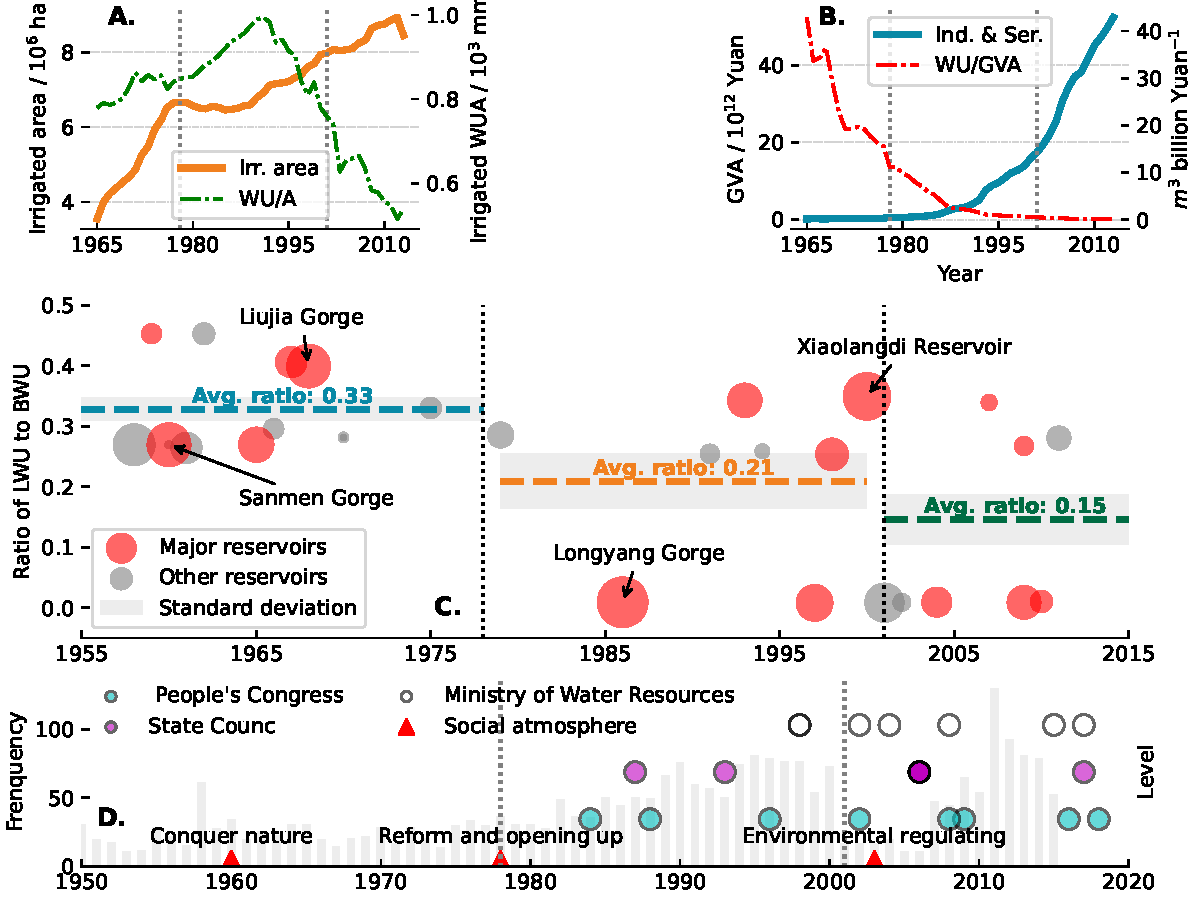
\includegraphics[width=\linewidth]{../../figures/main/causes.pdf}
	\caption{
		Causes of water governance regime shifts: environment changes, economic growths and efficiency changes, social transformation and water governance policies.
		\textbf{A.} Changes of total irrigated area, and water consumptions in per unit of area (\textit{SI Method} S2).
		\textbf{B.} Changes of gross values added (GVA) of industry and services, and their water use density (WUI) respectively (\textit{SI Appendix} Method S2).
		\textbf{C.} Completed time of each new reservoir and their located regions' water use percentages in basin's total water use (WU), at that time. Red ones denote hub reservoirs in the basin, which plays a role in basinal integrated water management. Size of the points indicates their magnitude of water storage capacities. Some important or special reservoirs' name denoted: (1) Xiaolangdi reservoir and Sanmen Reservoir were constructed mainly responsible for managing sediments of the Yellow River. (2) Liujia Gorge, Longyang Gorge, were constructed mainly responsible for managing water flood discharge and storage. These marked reservoirs, therefore are significant for the entire basin, far crucial than regional development.
		\textbf{D.} Social transformations and national levels' policies related to water governance (see \textit{Appendix SI} Table S2). Four transformations are ``ethos of overcome nature since 1958'', ``reform and opening-up since 1978'', ``the 87 Water Diversion Scheme since 1987'', ``environmental regulation since 2003'' in order.
	}
	\label{fig:Causes}
\end{figure}

% 经济总量提升导致资源耗竭的加速。
Firstly, the expansion of irrigated area and the economic growth of industry and services are keys to the changes in the provision between P1 and P2 (Figure\ref{fig:Causes}A). During the P1, irrigated agricultural area in the Yellow River basin expanded rapidly at a rate of $0.25*10^6 ha/yr$, and irrigation water was the dominant water use ($81.56\%$ of the total water use in 1965, and $83.17\%$ in 1978, see \textit{SI Appendix} Fig. S7). Entering P2, however, while the expansion of irrigated area stalled, industry and services gradually took off and took up more water resources (Figure\ref{fig:Causes} B), leading to $8\%$ reduction of proportion of irrigation water (\textit{SI Appendix} S7).

% 用水关系的变化
Secondly, efficiency of water use changed from the P2 to the P3.
While irrigated area resumed expansion again in the P3 whose water consumptions were still dominant (Figure\ref{fig:Causes} A), both industry, urban services were boosting their gross added values (GVA) (Figure~\ref{fig:Causes}B). 
However, the water use density (WUI) of them experienced significant declines and reached the lowest points (Figure~\ref{fig:Causes}A and Figure~\ref{fig:Causes}B).
It means, water governance have changed, along with technological solutions and a range of water conservation practices (\textit{SI Appendix} Fig. S8). As a result, the differences between the sectors of water use reduced while the total water consumption remains stable, during the P3 (\textit{SI Appendix} Fig. S7).

% 最后,环境背景、社会转型和水治理政策在这三个时期都发挥了作用。
Finally, environmental context, social transformation and water governance policies played roles throughout all three periods. 
% 根据水库的位置,计算了各水库的区域用水量与盆地用水量之比。
According to locations, we calculate the ratios of regional and basinal water use for each reservoir (R/B ratio), and a higher ratio represents potential role for storage rather than regulating (see \textit{SI Appendix} Figure S3).
% 在自然水资源相对丰富的P1年,水库大多建在需水量高的地区,水库的需水量比显著偏高。
Under the guide of ``ethos of overcome nature'', most of the reservoirs are built in regions with high water demands during the P1, when natural water resource is relatively abundant, as R/B ratios are significantly higher (Figure~\ref{fig:Causes}C, p<0.01). 
% 在P2中,新水库的数量显著减少,水量分配受到“87调水方案”的严格控制,总库容几乎没有增加(\textit{SI  Appendix}图S6)。
In the P2, the number of new reservoirs decreases significantly and allocation of water were rigorously controlled by ``the 87 Water Diversion Scheme'', with little increment of total storage capacities (\textit{SI Appendix} Fig. S6). 
% 而进入P3期后,新增水库数量远高于P1期,且多数建在区域用水量比较低的区域(图~\ref{fig: Causes}C和\textit{SI  Appendix}图S6)。
Entering the P3, myriad national-level water governance policies proposed under the guide of ``environmental regulation'', and the number of new reservoirs are even higher for facilitating regulation, most of which were built in regions with lower R/B ratio (Figure~\ref{fig:Causes}C and \textit{SI Appendix} Fig. S6).


% tag 讨论
\section*{Discussion}
\label{Discussion}

\subsection*{Water governance challenges along transition regimes}

\begin{figure*}[htbp!]
	\centering
	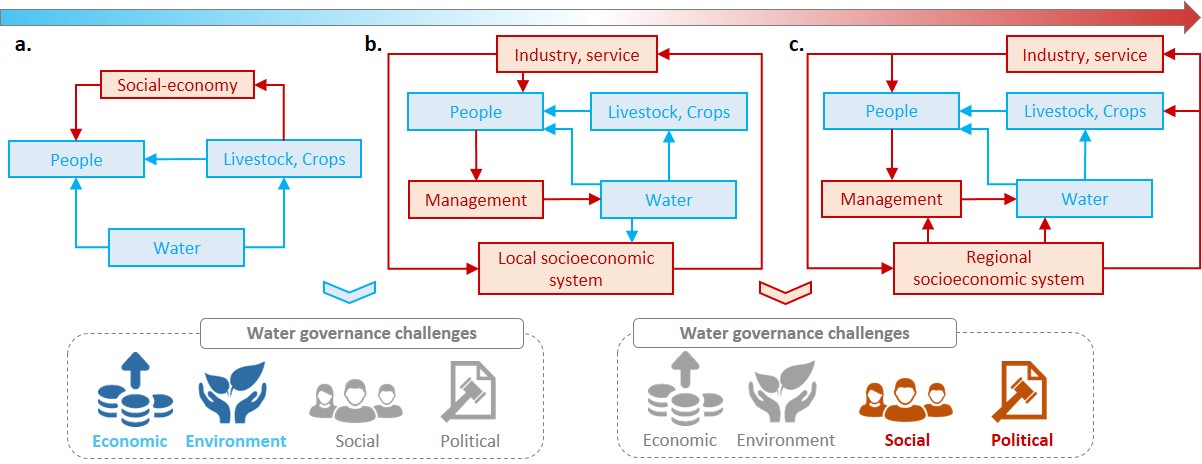
\includegraphics[width=\linewidth]{../../figures/main/transition.jpg}
	\caption{
		\textbf{Transition schema of water governance.} Blue pathways dominated by natural water loop while red ones dominated by socio-economic loops. There is a transformation towards the hydro-social water cycle where red loop increases.
		\textbf{A. Natural phase:} As an indispensable provisioning resource, the main functions of water resource is to support crop, livestocks and human-beings, which are the basic ecological services.
		\textbf{B. Local phase:} With local socio-economic systems developing, industry and services (also known as the secondary and the tertiary industry) calling for further water consumptions. What's more, better organized socio-economic system and developed technology gives humans abilities in better managing water resources, with intensive intervention in the natural water cycle. 
		\textbf{C. Regional phase:} With further developed and economically efficient industries and services, trade-off between whose water demands with provisional water demands becomes prominent. Rather than determined by local socio-economic systems, water withdrawals and management act as considerations within the entire basin more, therefore. 
		Water governance faces primarily economic and environmental challenges in the early stages while social and policy challenges in the later stages.
	}
	\label{fig:summary}
\end{figure*}

% 我们发明的指数能同时关注水资源治理的三个关键方面。
The IWGI index we developed captures three key dimensions of water governance simultaneously: (storage, provision and allocation). 
% 我们为的研究结果表明,黄河流域能被识别为三个明显的稳态。
Based on that, our results show that three distinct but sequential governance regimes within YRB, whose shifts have been caused by different environmental, economic, social or political aspects.
% 值得注意的是,这些多方面的变化随着流域逐步迈向水-社会循环的过程中逐步发生的,且在早期主要带来经济、环境方面的挑战,而后期则带来社会和政策方面的挑战。
It is important to note that these regimes with multifaceted causes occurred gradually as the basin moves towards a hydro-social cycle, facing primarily economic and environmental challenges in the early stages while social and policy challenges in the later stages (Figure~\ref{fig:summary}).

% 第一种时期(1965-1978年),流域经济以农业为主,自然水资源相对丰富,用水治理倾向于为农业提供更多的资源。
At the first regime (1965-1978), since the basin economy was mainly dependent on agriculture and natural water resources were relatively abundant in this period, governance of water use tended to provide more resources for agriculture (construction of reservoirs and channels for examples). 
% 因为此时社会经济对自然水循环的影响尚且有限,几乎没有保护政策的治理体系鼓励在需供水的地区进行无节制的取水和蓄水,而很少考虑流域的社会公平。
Due to the limited socio-economic influences on the natural water cycle, the governance system with few protective policies encouraged unlimited water withdrawals and storage in the regions requiring water supply, with little consideration of the social equity over the basin. 
% 近80%的地表水用于供应(家庭用水、牲畜用水或粮食生产),黄河的干涸发生在政权末期,留下了巨大的环境危机。
With nearly 80\% of surface water used for provisioning (domestic, livestocks' use or food production), drying up of the Yellow River occurred at the end of the regime and left a huge crisis of environment.

% 第二个政权与中国的经济改革相吻合,新兴的工业和服务业打破了农业的主导地位,在新的治理体制下争夺用水。
The second regime coincided with Chinese economic reform, when the emerging industry and services broke the dominance of agriculture and competed for water use under the new governance regime. 
% 与此同时,黄河水利委员会进行了改组,接到水利部(原水电部)的指示,恢复和加强黄河水利委员会的水文、流域管理工作。
At the same time, the Yellow River Conservancy Commission undergone a reorganization and received instructions from the Ministry of Water Resources (called Ministry of Water Resources and Electric Power then) to resume and strengthen work related to hydrology and basin management in YRB.
% 该制度稳态不仅遏止了用水效率低下的农业的扩张,更出台了一系列政策法规应对水资源压力,并调节用水分配。
As results, the regime not only stopped the expansion of inefficient agriculture, but also introduced a range of policies and regulations to deal with the stresses of water use and regulate the allocation of water.

% 第三次稳态转换直到1993年左右才由用水效率的显著提升而带来,因为社会经济发展后先进技术的广泛应用。
The next regime shift was not brought until a significant increase in water use efficiency around 1993, due to the widespread applying of advanced technologies after socio-economic developments. 
% 而区域社会经济的权衡成为了用水分配的关键,如此时期普及开的水权转换项目就是把节约的农业用水用于工业发展。
The regional socio-economic trade-off had become the key to water governance in this period, and for an example, the water rights conversion project popularized in this regime is to use the saved agricultural water for industrial developments.
% 但是曾帮助流域摆脱环境危机的分水政策却在此时期成为了流域协调和社会公平的桎梏。
However, the water allocating policy (i.g. ``87 Water Diversion Scheme''), which had helped the YRB get rid of the environmental crisis at the last regime, became the shackle of equity and coordination during this period.
% 这是因为用水分配方案高度路径依赖,用水方式也更加不灵活,这些成为新的社会经济形势下的治理难题。
This is because the water allocation scheme is highly path dependent and the way of water use is also more inflexible, both of which have become challenges for governance under the new regime.

% 总的来说,三个水治理稳态之间的先后转变,都是随着流域向社会-水循环发展的过程中先后发生的,存在明显的过渡趋势。
In general, shifts of the three governance regimes occurred sequentially with the transformation towards the hydro-social cycle, with an obvious transition.
% 随着不断增强的人类压力在全球普遍逐渐占据主导,这种过渡趋势在社会-生态系统中被认为是普遍存在的,例如生态系统服务和国家经济-社会发展。
This transition is considered to be pervasive in socio-ecological systems, such as ecosystem services and national economic-social developments, as increasing anthropogenic pressures gradually dominate the world at large.
% 流域转向社会-水循环的过程就是典型的社会-生态系统过渡过程,而我们发现在这一过程中水治理的稳态转换呼应了全球水治理面临的两大主要挑战。
With the typical transition towards a hydro-social water cycle, we find that the regime transition of water governance echoes the two kinds of major challenges globally.
% 根据前人广泛的总结,目前全球一部分流域正面临着经济发展和资源困境(如缺水和用水困难),而另一些则迫切需要社会政策层面的协调与合作以实现可持续(如跨境河流的用水分配与协作治理)。
According to the summary of previous studies, some river basins are facing economic development and resource dilemma (such as water shortage and water supplying difficulties), while others are in urgent need of coordination and cooperation at the social policy (such as water disputes and lack of cooperative governance, especially for cross-border rivers).
% 非常具有代表性的是,这两类主要挑战在黄河流域快速变迁的过程中先后发生了,伴随着整合了四个维度的(经济、环境、社会、政策)治理稳态的转换。
It is very representative that these two kinds of major challenges have occurred successively in the transition of the YRB, accompanied by the transformation of governance regime.
% 我们的分析表明,过渡的前期常常带来环境和经济层面的治理挑战,而在过渡的后期则主要是社会和政策层面的挑战。
Our analysis indicates that the early stage of transition often brings environmental and economic governance challenges, while the later stage of transition is dominated by social and policy challenges.
% 再一次,我们总结的框架呼应了联合国发展属为水治理提出的四个维度和两大主要问题。
Again, this schema outlines the key dimensions proposed by UNDP and two types of global challenges, regarding water governance. 


\subsection*{Implications and future directions}
\label{Outlook}

% 我们发展的指数捕捉了水治理的过渡制度,以一种相对全面但简单的方式
The index we developed (IWGI), captures the transition regimes of water governance with different challenges, in a relatively simple but comprehensive way.
% 对可持续科学家来说,认识到治理挑战的变化非常重要,因为发展不是解决一切的灵丹妙药。
It is important for scientists and decision makers to recognize the changing challenges for water governance, because development is not a panacea for all basin issues regarding sustainability.
% 对于当今世界来说,水资源供应压力不断增大仍然是全球最大的水治理挑战,而经济优先的策略仍然是应对挑战的主要方式。
For today's world, increasing water stresses on water use remains one of the greatest water governance challenges, while economic development provision strategies are still the main guideline to meet them. 
% 尽管绝大多数的大河流域都在快速发展的同时极大提高了管理水资源的能力和用水的效率,但大部分研究仍悲观的指出淡水利用已经临近系统崩溃的行星边界。
Although most large river basins improved water management and efficiency along with development, most studies still pessimistically point out that freshwater use is reaching planetary boundaries where human-water systems may collapse.
% 总的来说,这可能有两点主要原因。
Overall, there are probably two main reasons.
% 首先,效率悖论
Firstly, significant improvement in agricultural irrigation efficiency is usually accompanied by re-expansion in irrigated area, resulting in a usually unabated trend of water resources stress which is known as paradox of efficiency 
\cite{graftonParadoxIrrigationEfficiency2018}. 
% 其次,以水-社会水循环为主导的治理机制下,水资源分配或提供结构复杂,可能导致水资源利用不灵活,破坏流域的恢复能力
Secondly, complicated structure of water allocation or provision under a governance regime dominated by hydro-social water cycle may lead the water governance more inflexible and damage to resilience of the basin
\cite{qinFlexibilityIntensityGlobal2019}.
% 这时,我们需要相应的全面策略应对这种治理挑战,因为挑战的核心要素超出了任何一个参与的控制。
At this point, we need corresponding comprehensive strategies to address the governance challenges, because the heart factors of are beyond the control of any related actor. 
% 基于对治理体制转型对理解,我们可以创造有利条件以应对挑战,并保持流域社会-生态系统对弹性,以实现可持续发展。
Based on the understanding of governance regime transition, we can create favourable conditions for meeting the challenges and maintaining the resilience of the basin's socio-ecosystem, towards sustainability.
% 总的来说,这些都有助于指导流域迈向可持续性。
% Taken together, these have helped guide the basin towards sustainability.

%tag 研究方法
\matmethods{
Here, we constructed the Integrated Water Resources governance (IWGI) Index which consists of three dimensions and identified the changes periods of the index over time by change points detection. 
Each dimension is reflected by an independent indicator after normalization, and water governance regime were characterized by combination of impacts of each dimension in periods.
In addition, the contribution to changes of IWGI index along with each main indicators were decomposed and calculated separately for each regime (i.e. period). 
	
	\subsection*{Integrated Water Resources governance (IWGI) Index}
	% 我们认为水资源利用制度,与水资源利用的三个维度紧密相关:
	Water resources governance system is closely related to the social developments in three dimensions below (see \textit{SI Appendix} Methods S4 for details):
	
	% - 社会的发展通常伴随着用水向社会经济系统倾斜,用水方式优先向收益更高的非供给性方式倾斜:
	\begin{itemize}
		\item Social development is usually accompanied by a change of provision in water use towards social and economic systems because of higher returns:
		$$ Dev. \propto P $$
		% - 社会发展通常伴随着更具结构性的水资源配置,如区域部门之间的分工合作,以及区域的统筹配置:
		\item Social development usually lead to more complex structure in allocation of water resources, which is a result of division and cooperation between regions and sectors for developing:
		$$ Dev \propto A $$ 
		% - 可持续的社会发展应该通过技术手段有效缓解发展过程中产生的水资源压力,才能实现可持续发展:
		\item Further social development can only be achieved by effectively alleviating the water resource stresses generated in the process of development through technological means:
		$$ Dev \propto S^{-1} $$
	\end{itemize}
	
	% 将三者合一起,即:
	We combine the above three dimensions for an integrated index, remaining their positive or negative relationship with social development: 
	$$ Dev. \propto P*A*S^{-1} $$

	% 在上述假设的基础上,我们要构建流域综合耦合指数(Integrated Water Resources governance, IWGI),使 IWGI 有效表征与用水相关的三个维度。首先为每个维度选择一个合适的指示因子(indicator, $I_x$, 其中$x=P, C or S$)。将上式进行自然对数转换,从而让三个维度之间变成加减关系:
	To effectively represent the three dimensions, we select an appropriate indicator ($I_x$, $x=P$, $C$ or $S$ corresponding to provision, allocation and Stress respectively) for each dimension. Then, the above equation is transformed into a natural logarithm to facilitate calculation:

	$$ Dev. \propto ln(I_P) + ln(I_A) - ln(I_S) $$

	Assuming they have equal weights, the Integrated Water Resources governance (IWGI) Index:

	$$ IWGI = I'_A + I'_P - I'_S $$

	where $I'_x$ is a normalization of log-transformed indicator $I_x$ for a certain dimension:

	$$ I'_x = normalize(ln(I_x)) $$
	
	\subsubsection*{Normalization}
	In fact, we have tested different normalization methods and it makes no difference in change points detection (see \textit{SI Appendix} Methods S5. Sensitivity analysis). In this study, finally, we performed min-max normalization as the formulation below:

	$$ normalize(X) = (X - X_{min}) / (X_{max} - X_{min}) $$

	\subsubsection*{Indicator of Stress}
	We refer to the scarcity-flexibility-variability (SFV) water stress index proposed in Qin et al., 2019 to evaluate water stress ($SFV_i$) as the indicator in a certain region $i$ \cite{qinFlexibilityIntensityGlobal2019}. This metric takes into account management measures (such as the construction of reservoirs) and the impact of changes in the industrial structure of water use on the evaluation of water scarcity (see \textit{SI Appendix} Methods S4 for details). For the whole YRB, indicator of stress $I_S$ is the average stress of all regions' SFV-index: 

	$$ I_S = \frac{1}{4} * \sum_{i=1}^4 SFV_{i} $$
	
	Where $SFV_i$ is the SFV-index for region $i$, and $i=1$ to $4$ refers SR, UR, MR, and DR (see \textit{SI Appendix} Methods S1 Definition of study area).

	\subsubsection*{Indicator of provision}
	To provision $I_P$, we use Non-Provisioning Shares (NPS) of water use as an indicator. While provisional water use ($WU_{pro}$) includes domestic, irrigated and livestock water uses, the non-provisioning water use ($WU_{non-pro}$) includes industrial and urban services water uses. Then, we can calculate the non-provisioning shares by:

	$$ NPS_{i} = \frac{WU_{non-pro, i}}{WU_{pro, i} + WU_{non-pro, i}} $$

	Where $i$ refers a certain region, or the whole basin, i.e:

	$I_P$ = $NPS_{basin}$

	\subsubsection*{Indicator of allocations}
	%$CEM$ 指标度量的是水资源配置“不均匀”的程度,类似于信息熵是对“混乱程度”的度量,即参与分配的各个单位之间,分配比例差距越大,则熵越小。
	% 而我们的指标应反映随着社会发展,水资源配置在区域之间更加均衡(比例差距小)、整体满足不同用水部门的发展需求(比例差距减小)、但不同区域存在部门分工(比例差距增大)的趋势。
	To description of allocations $I_C$, we designed an indicator by imitation of information entropy, called allocation Entropy Metric (CEM), a metric to measure the degree of evenness of water allocation (see \textit{SI Appendix} Methods S4).
	While our indicator $I_C$ should reflect that with the development of society, water resources allocation is more balanced among regions and generally meets the needs of different sectors (means smaller gaps, too), but different regions have a trend of division of labour among various sectors (with larger gaps):

	$$ I_C = \frac{CEM_{r}*CEM_{s}}{CEM_{rs}}$$
	
	where $CEN_{r}$ and $CEN_{s}$ are allocation Entropy Metric in different regions and different sectors. $CEN_{rs}$ is differences between sectors in a certain region to the whole basin (see \textit{SI Appendix} Methods S4). 

	\subsection*{Change points detection}
		% The method makes no assumptions about the distribution of the data and detects breakpoints based solely on the probability of the data coming from different distributions before and after the breakpoint.

		With no assumptions about the distribution of the data, the Pettitt (1979) approach of changing points detection is commonly applied to detect a single change-point in hydrological series with continuous data \cite{pettittNonParametricApproachChangePoint1979}. 
		It tests the $H0$: The variables follow one or more distributions that have the same location parameter (no change), against the alternative: a change point exists. The non-parametric statistic is defined as:
	
		$$ K_t = max|U_{t, T}|$$

		Where:

		$$ U_{t, T} = \sum_{i=1}^t\sum_{j=t+1}^T sgn(X_i - X_j) $$
	
		The change-point of the series is located at $K_T$, provided that the statistic is significant. We use 0.001 as the threshold  of p-value (see \textit{SI Appendix} Methods S5 for Sensitivity analysis), which means the probability of a statistically significant change-point judgment being valid is more than $99.9\%$.
		Since this method only can return one significant change point, we repeat it Until all significant change points were detected.
	
	% 计算贡献度
	\subsection*{Contribution decomposition}
		We have decomposed the amount of variation in each index at different stages in order to observe the contribution of each influencing factor to them. Use Integrated Water Resources governance (IWGI) Index as an example, which influenced by three dimensions' normalized indicator: stress ($I'_S$), provision ($I'_P$) and allocation ($I'_C$). We can calculate their differences between two certain years ($y_2$ and $y_1$, $y_2 > y_1$) by:

		\begin{align*}
			\Delta IWGI &= (I'_{P_{y_2}} + I'_{C_{y_2}} - I'_{S_{y_2}}) - (I'_{P_{y_1}} + I'_{C_{y_1}} - I'_{S_{y_1}}) \\
			&= (I'_{P_{y_2}} - I'_{P_{y_1}}) + (I'_{C_{y_2}} - I'_{C_{y_1}}) + (I'_{S_{y_1}} - I'_{S_{y_2}}) \\
			&= \Delta I'_P + \Delta I'_C + (-\Delta I'_S)
		\end{align*}
		Then, the contribution of dimension $x$ to IWGI's changes can be referred as:

		$$ Contribution_x = \frac{\Delta I'_x}{|\Delta IWGI|} $$

		% Since $Contribution_x$ can be positive or negative, we used an absolute value to evaluate the contribution (in proportion) of a certain dimension in the all three dimensions to the changes:
		% $$  Contribution_x\% = \frac{|\Delta I'_x|}{\sum_x |\Delta I'_x|} $$

		% or just for contributions (in proportion) within a certain year $j$ to the regime:
		% $$ Contribution_{x,j}\% = \frac{|I'_{x, j}|}{|\sum_x I'_{x, j}|} $$

	\subsection*{Datasets}
	% 为了计算 IWGI ,我们需要计算多个指标及子指标,所有使用的数据集都在表中列出,数据的详细介绍可见补充材料。
	In order to calculate IWGI, we need to calculate multiple indicators and sub-indicators. All the datasets used are listed in the \textit{SI Appendix} table S1. A detailed description of the data can be seen in the supplementary materials \textit{SI Appendix} Methods S2.
}

\showmatmethods{} % Display the Materials and Methods section

\acknow{Please include your acknowledgments here, set in a single paragraph. Please do not include any acknowledgments in the Supporting Information, or anywhere else in the manuscript.}

\showacknow{} % Display the acknowledgments section

% Bibliography
\bibliography{my-papers}
	
\end{document}